\chapter{Authentifizierung und Autorisierung}
Um den Zugriff auf Zielsystem und REST-API gleichermaßen zu steuern und dabei im Zielsystem keine Anmeldeinformationen vorhalten zu müssen, wird eine Authentifizierung und Autorisierung per OAuth2-Protokoll und OpenID Connect vorgeschrieben.\\
\\
Der Ablauf der Autorisierung per OAuth2-Protokoll im Authorization-Code-Flow ist in der folgenden Grafik dargestellt \cite{rfc6749}. 

\begin{figure}[htbp]
\centering
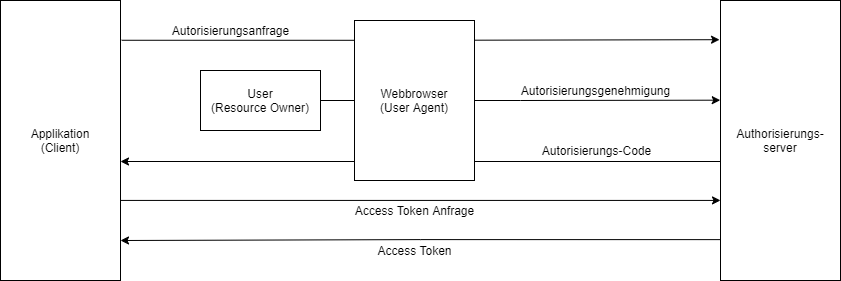
\includegraphics[width=\textwidth]{Authentication_Flow.png}
\caption{Access-Token-Erstellung im Authentication-Code-Flow}
\end{figure}

Über den Access Token erhält der Benutzer schließlich Zugriff auf das Zielsystem bzw. auf die REST-API, über den ID Token auf die ID (uuid) und ggf. weitere personenbezogene Daten des Benutzers. 
Sofern die personenbezogenen Daten für die Anlage eines Benutzerkontos (z.B. Vor- und Nachname, E-Mail-Adresse) benötigt werden, können diese durch die geeignete Wahl von scopes und claims im Aufruf der Autorisierungs-URL vom Resource Server abgefragt werden und initial zur Benutzerkontoerstellung genutzt werden.\\
\\
Der IDM-Provider muss dabei den Autorisierungsserver (OpenID Provider) und Resource Server zur Verfügung stellen, zudem müssen folgende Endpunkte definiert sein:\\

\begin{table}[htb]
    \begin{tabularx}{\textwidth}{|c|X|}
        \hline
\textbf{Endpunkt} & \textbf{Funktion des Endpunkts} \\ \hline
Autorisierung & Initiierung der Autorisierung und Benutzerzustimmung mit definierten Parametern (u.a. scopes/claims und Redirect-URL) \\ \hline
Token & Liefert ID und Access Token zurück \\ \hline
Revocation & Endpunkt, um den Access Token zu widerrufen \\ \hline
UserInfo & Kann definierte Benutzerdaten zur Verfügung stellen (z.B. uuid, Vor- und Nachname, E-Mail-Adresse) \\ \hline
    \end{tabularx}

        \caption{Endpunkte, die durch den IDM-Provider für die Anmeldung per OAuth2 in Verbindung mit OpenID Connect zur Verfügung gestellt werden müssen}
        \label{tab:auth:endpoints}
\end{table}

Die Spezifikation der REST-API sieht vor, dass die Sichtbarkeit der Daten an den definierten Endpunkte bereits im JSON-Objekt gemäß der Berechtigung des anfragenden Benutzers berücksichtigt ist. 
Die ID des Benutzers im Access Token allein reicht nicht aus, um die Sichtbarkeit der Daten korrekt zu beschränken, da einem Benutzer im IDM mehrere Institut-Rolle-Kombinationen zugewiesen sein können (z.B. an verschiedenen Institutionen als Lehrkraft tätig oder an derselben Institution sowohl Lehrkraft als auch Elternteil eines Schülers). 
Daher muss die Information, mit welcher Kombination von Institution und Rolle innerhalb dieser Institution der Aufruf eines REST-API-Endpunkts durchgeführt wird, an den IDM-Provider übermittelt werden. 
Dies geschieht durch die Erweiterung der Scopes-Liste (um jeweils den Scope für die Institution und die Rolle) als Parameterübergabe beim Autorisierungsvorgang. 
Die zusätzlichen Scopes für Institution und Rolle sind somit im Access Token hinterlegt und können bei der Generierung des zurückzuliefernden JSON-Objekts verwendet werden. \\
\\
Ein Sonderfall stellen dabei Benutzerkonten mit der Rolle ''sync-system'' dar. 
Diese haben bei Aufruf eines REST-API-Endpunkts grundsätzlich keine Beschränkung auf eine einzelne Institution. 
Um die Tokengenerierung zu vereinheitlichen, wird für Benutzerkonten mit der Rolle ''sync-system'' statt des Institutionsnamens die Bezeichnung der IDM-Domäne verwendet.\\
\\
Beispiel:

\begin{lstlisting}[caption={},frame=tlrb]
https://<URl zu Autorisierungsendpunkt>?response_type=code
&client_id=<Identifier von Client-App>
&redirect_uri=<Redirect-URL>
&scope=openid sync-system idm-domain
&state=<Undurchschaubarer Wert fuer Sicherheitszwecke>
\end{lstlisting}

Sofern für ein Benutzerkonto im IDM mehrere Institution-Rolle-Kombinationen hinterlegt sein können, müssen Institution und Rolle bei Start des Authentifizierungsprozesses gegebenenfalls durch den Benutzer wählbar sein. 
Für einen Instituiton-Rolle-Wechsel ist eine Neuanmeldung bzw. Aktualisierung des Access Tokens bezüglich der Scopes für Institution und Rolle notwendig. \\
\\
\\
Für den Logout bzw. Aktualisierungen aus dem IDM kann der Access Token am Autorisierungsserver widerrufen werfen (Token Revocation.)